\PassOptionsToPackage{sols}{handout}
\documentclass[main]{subfiles}
\setcounterrefbeforedot{chapter}{m-ws3-5}
\setcounterrefafterdot{section}{m-ws3-5}
\addtocounter{section}{-1}
\usepackage{solutions}

\begin{document}

\ifSubfilesClassLoaded{%
  \chaptermark{\chapterthree}
}{}

\section{Derivatives of Inverse Trig Functions} \label{ws3-5}

\begin{problemonly}
    \begin{framed}

\textbf{Key Ideas}:

\begin{itemize}[topsep=0pt,partopsep=0pt,parsep=8pt,itemsep=0pt]

\item You should be able to find the derivatives of the inverse
  trigonometric functions using implicit differentiation.  You should be
  able to apply the same strategy to other inverse functions (try it out
  with $e^x$ and $\ln x$, for instance.)

\item You should know the derivatives of $\arcsin x$, $\arccos x$,
  $\arctan x$ and be able to use these to solve problems. 

\item You should be able to reason about the compositions of trigonometric
  and inverse trigonometric functions such as $\cos(\arctan x)$ and
  $\sin(\arcsin x)$. You should be able to determine the domains of such
  functions as well as to simplify them.

\end{itemize}
\end{framed}
\end{problemonly}

\begin{enumerate}
\item 
  \begin{enumerate}
  \item
    \begin{problem}[\vfill]
      Sketch $y = \arctan x$, and label any horizontal and vertical
      asymptotes on your graph.  Then, sketch a rough graph of the
      derivative of $\arctan x$.
    \end{problem}

    \begin{solution}
      Here is the graph of $\arctan x$:
      \begin{center}
        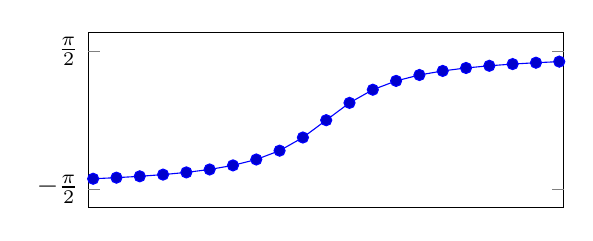
\begin{tikzpicture}
          \begin{axis}[xtick=\empty, ytick=\empty, extra y ticks={-1.5708,
              1.5708}, extra y tick labels={$-\frac{\pi}{2}$,
              $\frac{\pi}{2}$}, xmin=-4.25, xmax=4.25, width=3in,
            height=1.5in, ymin=-2, ymax=2] % 
            \addplot+[blue, solid]{rad(atan(x))};
          \end{axis}
        \end{tikzpicture}
      \end{center}
      The domain is $(-\infty, \infty)$, and the range is
      $\left(-\frac{\pi}{2}, \frac{\pi}{2} \right)$.
    \end{solution}

  \end{enumerate}
  Now, we'll find the derivative of $y = \arctan x$.  
  \begin{enumerate}[resume]
  \item
    \begin{problem}[0.25in]
      Rewrite the equation $y = \arctan x$ as an equation involving
      $\tan$ rather than $\arctan$.
    \end{problem}

    \begin{solution}
      We can rewrite the equation $y = \arctan x$ as $\tan y = x$.  
    \end{solution}

  \item
    \begin{problem}[1in]
      Use implicit differentiation on your equation from part (b),
      to find $\diff yx$. 
      
      
    \end{problem}

    \begin{solution}
      We differentiate both sides of the equation $\tan y = x$ with
      respect to $x$: 
      \begin{align*}
        \frac{d}{dx} (\tan y) &= \frac{d}{dx} (x) \\
        \sec^2 y \cdot \frac{dy}{dx} &= 1 \\
        \frac{dy}{dx} &= \cos^2 y 
      \end{align*}
    \end{solution}

    \note{Matt note - This particular step can be a tricky jump, mainly because students really want to know what the angel $y$ is, when in reality, we just need the cosine of it.}

    \item 
    \begin{problem}[\vfill\newpage]
        From part (c), you should have some expression in terms
      of $\cos y$, but we want $\diff yx$ in terms of $x$. Use your answer for part (b), along with an appropriate right triangle, 
      to express $\diff yx$ in terms of $x$.

      Does your final answer match the graph you sketched in part (a)?
    \end{problem}

    \begin{solution}
        Although we now have an expression for $\frac{dy}{dx}$, this isn't a
      good answer to the original question.  We were asked for the
      derivative of a function of $x$, so our answer ought to be in terms
      of $x$.  Remember that $y = \arctan x$; that is, $y$ is the angle in
      $\left( - \frac{\pi}{2}, \frac{\pi}{2} \right)$ whose tangent is
      $x$.  We can draw a picture of this statement:
      \begin{center}
        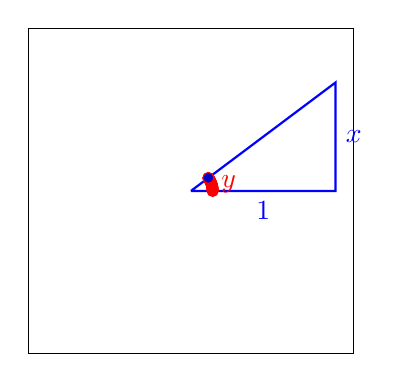
\begin{tikzpicture}
          \begin{axis}[axis equal=true, xmin=-4.5, xmax=4.5, ymin=-4.5,
            ymax=4.5, xtick=\empty, ytick=\empty, width=2.25in,
            height=2.25in, clip=false] %
            \draw[blue, thick] (axis cs: 0, 0) -- node[below]{$1$} (axis cs:
            4, 0) -- node[right]{$x$} (axis cs: 4, 3) -- (axis cs: 0, 0); %
            \pgfmathsetmacro{\angle}{atan(3/4)} %
            \addplot+[domain=0:\angle, red, thin, ->, >=to] ({0.6 *
              cos(x)}, {0.6 * sin(x)}) node[pos=0.5, right] {$y$};
          \end{axis}
        \end{tikzpicture}        
      \end{center}
      By the Pythagorean Theorem, the triangle has hypotenuse $\sqrt{1 +
        x^2}$, so $\cos y = \frac{1}{\sqrt{1 + x^2}}$, and $\displaystyle
      \frac{dy}{dx} = \cos^2 y = \boxed{\frac{1}{1 + x^2}}$.
    \end{solution}

  \end{enumerate}

\item 
  \begin{problem}
    In this problem, you'll find the derivative of $\arcsin x$.
    \begin{enumerate}[topsep=0pt]
      \item 
        \begin{problem}[0.5in]
        Rewrite $y=\arcsin x$ as an equation involving sine.
        \end{problem}

      \item
        \begin{problem}[0.75in]
        Differentiate implicitly to find $\diff yx$.
        \end{problem}

    \item
      \begin{problem}[1.5in]
      Express $\diff yx$ in terms of $x$ only, using the same technique from \#1(d).
      \end{problem}
    \end{enumerate}
  \end{problem}

  \begin{solution}
    To find a formula for $\frac{d}{dx} (\arcsin x)$, we start with the
    equation
    \begin{align*}
      y &= \arcsin x \\
      \intertext{We'd like to find $\frac{dy}{dx}$, and we'll first
        rewrite this in terms of $\sin$ since we know how to differentiate
        $\sin$:}
      \sin y &= x \\
      \shortintertext{Differentiate both sides with respect to $x$:}
      \frac{d}{dx} (\sin y) &= \frac{d}{dx} (x) \\
      \cos y \frac{dy}{dx} &= 1 \\
      \frac{dy}{dx} &= \frac{1}{\cos y}
    \end{align*}
    As in {{\#1}}, we need to figure out how to express
    this in terms of $x$.  The equation $y = \arcsin x$ says that $y$ is
    the angle in $\left( - \frac{\pi}{2}, \frac{\pi}{2} \right)$ whose
    sine is $x$, and we can picture this statement graphically:
    \begin{center}
      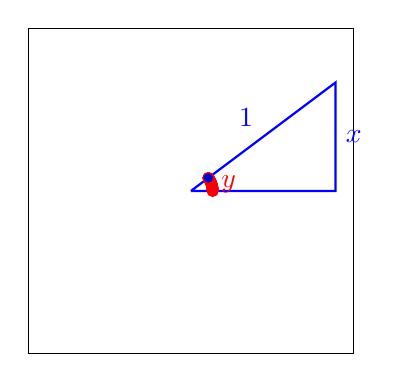
\begin{tikzpicture}
        \begin{axis}[axis equal=true, xmin=-4.5, xmax=4.5, ymin=-4.5,
          ymax=4.5, xtick=\empty, ytick=\empty, width=2.25in,
          height=2.25in, clip=false] %
          \draw[blue, thick] (axis cs: 0, 0) -- (axis cs: 4, 0) --
          node[right]{$x$} (axis cs: 4, 3) -- node[anchor=south east]
          {$1$} (axis cs: 0, 0); %
          \pgfmathsetmacro{\angle}{atan(3/4)} %
          \addplot+[domain=0:\angle, red, thin, ->, >=to] ({0.6 *
            cos(x)}, {0.6 * sin(x)}) node[pos=0.5, right] {$y$};
        \end{axis}
      \end{tikzpicture}        
    \end{center}
    By the Pythagorean Theorem, this triangle has width $\sqrt{1 - x^2}$,
    so $\cos y = \frac{\sqrt{1 - x^2}}{1} = \sqrt{1 - x^2}$.  Therefore,
    $\displaystyle \frac{dy}{dx} = \frac{1}{\cos y} =
    \boxed{\frac{1}{\sqrt{1-x^2}}}$.
  \end{solution}

\end{enumerate}

  \begin{framed}
    \textbf{Derivatives of the inverse trigonometric functions.}  (You
    should memorize these.)
    
      $\displaystyle \frac{d}{dx} (\arcsin x) = \fitb{1in}{\displaystyle
        \frac{1}{\sqrt{1 - x^2}}}$

      $\dfrac{d}{dx} (\arccos x) = - \dfrac{1}{\sqrt{1 - x^2}}$

      $\dfrac{d}{dx} (\arctan x) = \fitb{1in}{\displaystyle \frac{1}{1 +
          x^2}}$

    (You'll do $\arccos x$ on your homework.)
  \end{framed}


\begin{enumerate}[resume]

\item 

  Differentiate the following functions.  (You should \emph{not} need
  implicit differentiation here; rather, use what you already know about
  the derivatives of $\arcsin x$, $\arccos x$, and $\arctan x$.)
  \begin{enumerate}
  \item
    \begin{problem}[\vfill]
      $f(x) = \displaystyle \arcsin \left( \frac{1}{x} \right)$
    \end{problem}

    \begin{solution}
      We use the Chain Rule with $\frac{1}{x}$ as the inner function:
      $\displaystyle f'(x) = \boxed{\frac{1}{\sqrt{1-\left(\frac{1}{x}
            \right)^2}}\cdot \left(- x^{-2} \right)}$.
    \end{solution}

  \item
    \begin{problem}[\vfill]
      $g(x) = \displaystyle e^{3x} \arccos(2x)$
    \end{problem}

    \begin{solution}
      We first need the Product Rule:
      \begin{align*}
        g'(x) = {} & \frac{d}{dx}
        \left(\fcolorbox{green}{white}{$\displaystyle  e^ { 3 x} $}\cdot
          \fcolorbox{green}{white}{$\displaystyle  \arccos\left(2
              x\right)$}\right) \\
        = {} & e^ { 3 x} \cdot \frac{d}{dx} \left(\fcolorbox{red}{white}{$\displaystyle \arccos\left(\fcolorbox{blue}{white}{$\displaystyle 2 x$}\right)$}\right)+ 3 e^ { 3 x} \cdot \arccos\left(2 x\right) \\
        = {} & \boxed{e^ { 3 x} \cdot \left(-\frac{1}{\sqrt{1-(2 x)^2}}\cdot
          2\right)+ 3 e^ { 3 x}  \arccos\left(2 x\right) }
      \end{align*}
    \end{solution}

  \item
    \begin{problem}[\vfill]
      $h(x) = \sqrt{\arctan (4x)}$
    \end{problem}

    \begin{solution}
      \begin{align*}
        h'(x) = {} & \frac{d}{dx}
        \left(\fcolorbox{red}{white}{$\displaystyle
            \fcolorbox{blue}{white}{$\displaystyle  \arctan\left(4
                x\right)$}^ { \frac{1}{2}} $}\right) \\ 
        = {} & \frac{1}{2} \cdot \arctan\left(4
          x\right)^ { -1/2} \cdot \frac{d}{dx}
        \left(\fcolorbox{red}{white}{$\displaystyle
            \arctan\left(\fcolorbox{blue}{white}{$\displaystyle 4
                x$}\right)$}\right) \\ 
        = {} & \boxed{\frac{1}{2}\cdot \arctan\left(4
          x\right)^ { -1/2} \cdot \left(\frac{1}{1 + (4x)^2}\cdot
          4\right)} 
      \end{align*}
    \end{solution}
  \end{enumerate}

\probonly{\newpage}


  \item 
 As you can see from the derivations above, it can be useful to be able to simplify expressions like $\cos(\arcsin x)$. Let's try
  some below. We will walk you through the first one.

  \begin{enumerate}[topsep=0pt]

    \item
      $\cos(\arcsin (-\frac{4}{5}))$
        \begin{enumerate}[topsep=0pt]
          \item Replace $\arcsin ({-\frac{4}{5}})$ with the equivalent
            expression in words:
            
            \fbox{cosine of (the angle in $[-\frac{\pi}{2},
            \frac{\pi}{2}]$ whose sine is $-\frac{4}{5})$.}

            \item
              \begin{problem}[\stretch{0.25}]
                Since $-\frac{4}{5}$ is negative, we know that
                (the terminal side of) the angle in question is in
                which quadrant? Based on that, what should the sign of your final answer be: positive or negative?
              \end{problem}

              
                The angle is in \fbox{quadrant IV,} since its sine is negative and
                the angle is in $[-\frac{\pi}{2},\frac{\pi}{2}]$.
                This means our final answer, which is the cosine of an angle,
                will be \fbox{positive.}
              

            \item
              \begin{problem}
                Draw a right triangle with acute angle $\theta$ where $\theta$
                is the reference angle. Label the lengths of the sides of the
                triangle so that $\sin \theta = |-\frac{4}{5}| = \frac{4}{5}$.
                Find the length of the remaining side using the Pythagorean Theorem.
                \fbox{
                \begin{tikzpicture}[scale=0.5]
                    \coordinate (O) at (0,0);
                    \coordinate (A) at (3,0);
                    \coordinate (B) at (3,4);
                    \draw (O) -- (A) -- (B) -- cycle;
                    \draw (2.4,0.6) rectangle (3,0);
                    \draw pic[draw=black,angle radius=15,
                    "$\theta$"] {angle=A--O--B};
                    \path (O) -- node[below] {$3$} (A) --
                    node[right] {$4$} (B) -- node[above left=-2pt] 
                    {$5$} cycle;
                \end{tikzpicture}}
              \end{problem}

            \item
              \begin{problem}[\stretch{0.25}]
                Find the cosine of this angle. This is the answer up to sign,
                and we can determine the correct sign based on step ii.
              \end{problem}


                Based on our triangle, $\cos \theta = \frac{3}{5}$. Since
                $\arcsin(-\frac{4}{5})$ is in quadrant IV, where cosine is
                positive, \fbox{$\cos(\arcsin(-\frac{4}{5}))=\frac{3}{5}.$}

        \end{enumerate}
    \item 
    $\sin(\arccos(-\frac{1}{3}))$
        \begin{enumerate}[topsep=0pt]
          \item
            \begin{problem}[0.25in]
              Write this in words.
            \end{problem}

            \begin{solution}
            Sine of the angle in $[0,\pi]$ whose cosine is $-\frac{1}{3}$.
            \end{solution}

            \item
              \begin{problem}[0.25in]
                In which quadrant is the relevant angle?
                What is the sign of your final answer?
              \end{problem}

              \begin{solution}
                The angle is in quadrant II, since its cosine is negative and
                the angle is in $[0,\pi]$. Sine of an angle in quadrant II is
                positive.
              \end{solution}

            \item
              \begin{problem}[\vfill]
                Draw the relevant right triangle and label all sides.
              \end{problem}

              \begin{solution}
              
                \begin{tikzpicture}[scale=0.7]
                    \coordinate (O) at (0,0);
                    \coordinate (A) at (3,0);
                    \coordinate (B) at (3,4);
                    \draw (O) -- (A) -- (B) -- cycle;
                    \draw (2.4,0.6) rectangle (3,0);
                    \draw pic[draw=black,angle radius=15,
                    "$\theta$"] {angle=A--O--B};
                    \path (O) -- node[below] {$1$} (A) --
                    node[right] {$\sqrt8$} (B) -- node[above left=-2pt] {$3$} cycle;
                \end{tikzpicture}
              \end{solution}

            \item
              \begin{problem}[0.25in]
                Determine your final answer.
              \end{problem}

              \begin{solution}
                Based on our triangle, $\sin \theta = \frac{\sqrt8}{3}$. Since
                our answer should be positive, \fbox{$\sin(\arccos(-\frac{1}{3}))=\frac{\sqrt{8}}{3}.$}
              \end{solution}
        \end{enumerate}

\probonly{\newpage}
  
    \item 
      \begin{problem}[\vfill]
        Simplify $\sin(\arctan x)$, where $x<0$.
      \end{problem}
      
      \begin{solution}
      $\arctan x$
      is the angle in $\left( - \frac{\pi}{2}, \frac{\pi}{2} \right)$
      whose tangent is $x$.  Since $x < 0$, $\arctan x$ must be in
      $\left( - \frac{\pi}{2}, 0 \right)$.  The relevant reference triangle
      looks like this:
      \begin{center}
        \begin{tikzpicture}[scale=0.7]
            \coordinate (O) at (0,0);
            \coordinate (A) at (3,0);
            \coordinate (B) at (3,4);
            \draw (O) -- (A) -- (B) -- cycle;
            \draw (2.4,0.6) rectangle (3,0);
            \draw pic[draw=black,angle radius=15,
            "$\theta$"] {angle=A--O--B};
            \path (O) -- node[below] {$1$} (A) --
            node[right] {$|x|$} (B) -- node[above left=-2pt]
            {$\sqrt{1+|x|^2}$} cycle;
        \end{tikzpicture}
      \end{center}
      (Note that we've called the length of the vertical side $|x|$
      because lengths should always be positive, and $x$ is negative.)  By
      the Pythagorean Theorem, this triangle has hypotenuse $\sqrt{1 +
        |x|^2} = \sqrt{1 + x^2}$, so the sine value of the angle
      $\arctan x$ is $- \dfrac{|x|}{\sqrt{1 + x^2}}$.  But since $x$ is
      negative, $-|x|$ is just $x$, so we can more simply say that $\sin
      \left( \arctan x \right) = \boxed{\frac{x}{\sqrt{1 + x^2}}}$.
    \end{solution}
    
  \end{enumerate}



\item 
  In this problem, you'll graph $f(x) = \cos(\arccos x)$.
  \begin{enumerate}
  \item
    \begin{problem}[0.25in]
      What is the domain of $f$?
    \end{problem}

    \begin{solution}
      In order for $f(x)$ to be defined, we first need $\arccos x$ to be
      defined, which means $x$ must be in $[-1, 1]$.  If $\arccos x$ is
      defined, then $\cos(\arccos x)$ will also be defined, so the
      \fbox{domain of $f$ is $[-1, 1]$}.
    \end{solution}

  \item
    \begin{problem}[1in]
      For what values of $x$ is it true that $f(x) = x$?
    \end{problem}

    \begin{solution}
      $f(x)$ is only defined for $x$ in $[-1, 1]$.  If $x$ is any number
      in $[-1, 1]$, let $\theta = \arccos x$.  In words, $\theta$ is the
      angle in $[0, \pi]$ whose cosine is $x$ (that is, $\cos \theta =
      x$).  Then, \[f(x) = \cos \Big( \underbrace{\arccos x}_\theta \Big)
      = \cos \theta = x.\] So, \fbox{$f(x) = x$ for all $x$ in $[-1, 1]$}.
    \end{solution}

  \item
    \begin{problem}[\vfill]
      Compute $f'(x)$. Simplify completely. (You should get a constant. 
      Why does this make sense?)
    \end{problem}

    \begin{solution}
        We use the Chain Rule:
        \begin{align*}
        f'(x) &= \diff*{\outside{$\cos(\inside{$\arccos x$})$}}{x} \\
        &= -\sin(\arccos x) \cdot \frac{-1}{\sqrt{1-x^2}}
        \end{align*}
        To determine the value of $-\sin(\arccos x)$, we can picture it
        graphically. Let's say $y=\arccos x$.
    \begin{center}
      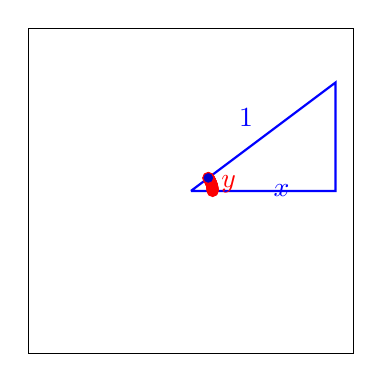
\begin{tikzpicture}
        \begin{axis}[axis equal=true, xmin=-4.5, xmax=4.5, ymin=-4.5,
          ymax=4.5, xtick=\empty, ytick=\empty, width=2.25in,
          height=2.25in, clip=false] %
          \draw[blue, thick] (0,0) -- node[right]{$x$} (4,0) --
           (4,3) -- node[anchor=south east]
          {$1$} (0,0); 
          \pgfmathsetmacro{\angle}{atan(3/4)} %
          \addplot+[domain=0:\angle, red, thin, ->, >=to] ({0.6 *
            cos(x)}, {0.6 * sin(x)}) node[pos=0.5, right] {$y$};
        \end{axis}
      \end{tikzpicture}        
    \end{center}
    By the Pythagorean theorem, $\sin y = \sqrt{1-x^2}$. This means that
    \[f'(x)=-\sin(\arccos x) \cdot \frac{-1}{\sqrt{1-x^2}}=\boxed{1}\]
    
        This makes sense because $f(x)=x$ on the entire domain $[0,1]$.
    \end{solution}

  \item

    \note{This is a good opportunity to get them to think about
      consistency.} 

    \begin{problem}[\vfill]
      Sketch the graph of $f$.  Clearly indicate the domain and range.
    \end{problem}

    \begin{solution}
      This is just a matter of putting the previous parts together.  We've
      seen that the domain of $f$ is $[-1, 1]$, and $f(x) = x$ for all $x$
      in $[-1, 1]$.  This tells us the graph of $f$:
      \begin{center}
        \begin{tikzpicture}
          \begin{axis}[xmin=-1.2, xmax=1.2, axis equal=true, width=2in,
            height=2in] 
            \addplot+[scatter, scatter src=explicit symbolic] coordinates
            {
              (1, 1) [closed]
              (-1, -1) [closed]
            };
          \end{axis}
        \end{tikzpicture}
      \end{center}      
    \end{solution}

  \end{enumerate}



  \probonly{\newpage}

\item In this problem, you'll graph $g(x)=\arccos(\cos x)$.

\begin{enumerate}[topsep=0pt]
    \item
      \begin{problem}[0.25in]
        What is the domain of $g$?
      \end{problem}

      \begin{solution}
      The \fbox{domain of $g$ is all real numbers}: if $x$ is any real
      number, $\cos x$ is defined and in $[-1, 1]$, so $\arccos(\cos x)$
      is also defined. 
      \end{solution}

    \item
      \begin{problem}[0.25in]
        What is the range of $g$?
      \end{problem}

      \begin{solution}
      The \fbox{range of $g$ is $[0,\pi]$}: if $x$ is any real
      number, $\cos x$ is defined and in $[-1, 1]$, so $\arccos(\cos x)$
      will be in $[0,\pi]$.
      \end{solution}

  \item
    \begin{problem}[1in]
      For what values of $x$ is it true that $g(x) = x$?
    \end{problem}

    \begin{solution}
      If $x$ is any number, let $a = \cos x$.  Then, \[ g(x) = \arccos
      \Big( \underbrace{\cos x}_a \Big) = \arccos a = \text{the angle in
        $[0, \pi]$ whose cosine is $a$}.\] This angle will only be $x$ if
      $x$ is in $[0, \pi]$, so \fbox{$g(x) = x$ for $x$ in $[0, \pi]$}.
    \end{solution}

  \item

    \note{The wording here is intentionally vague: the period of a
      periodic function can be difficult to determine, but they should
      understand that a function of the form $h(\cos x)$ must repeat every
      $2 \pi$ because $\cos x$ repeats every $2 \pi$.  (The period may be
      smaller than $2 \pi$, but we don't expect them to be able to
      determine what it is in general.)}

    \begin{problem}[0.5in]
      Is $g$ periodic?  If so, how often does it repeat?
      \emph{(If this is confusing, come back to it.)}
    \end{problem}

    \begin{solution}
      $g$ \fbox{is periodic} because it's a composition whose inner
      function (namely, $\cos x$) is periodic.  It \fbox{must repeat every
        $2 \pi$} because $\cos x$ does.  We can verify this by showing
      that $g(x + 2 \pi) = g(x)$:
      \begin{align*}
        g(x + 2\pi) &= \arccos (\cos (x + 2\pi)) \\
        &= \arccos(\cos x) \text{ since $\cos x$ repeats every $2\pi$} \\
        &= g(x) \checkmark
      \end{align*}
    \end{solution}
    

  \item

    \begin{problem}[\stretch{0.5}]
      If $x$ is in $[\pi, 2 \pi]$, what is $\arccos(\cos x)$?

      A good way to check yout answers is to try values you know,
      like $x=\pi$, $\frac{5\pi}{4}$, $\frac{7\pi}{4}$, or $2\pi$.
      Trying simple examples is a useful problem-solving skill!
    \end{problem}

    \begin{solution}
      Since the inner function is $\cos x$, it makes sense to think of $x$
      as an angle in $[\pi, 2 \pi]$.  Let's sketch a couple of examples;
      here's one:
      \begin{center}
        \begin{tikzangle}[angle=7*pi/6, label=$x$, func=cos,
          functick=$\cos x$, labelpos=0.6]
        \end{tikzangle}
      \end{center}
      Then, $\arccos(\cos x)$ is the angle in $[0, \pi]$ whose cosine
      value is $\cos x$, so it must be the blue angle below:
      \begin{center}
        \begin{tikzangle}[angle=7*pi/6, label=$x$, labelpos=0.8, func=cos,
          functick=$\cos x$, secondangle=5*pi/6, secondlabel=$\arccos(\cos
          x)$, seconddistance=0.2, secondlabelpos=0.05]
        \end{tikzangle}
      \end{center}
      Here's another example showing a different angle $x$ in $[\pi,
      2\pi]$:
      \begin{center}
        \begin{tikzangle}[angle=3*pi/2+pi/6, label=$x$, func=cos,
          functick=$\cos x$, labelpos=0.4]
        \end{tikzangle}
      \end{center}
      Again, $\arccos(\cos x)$ is the angle in $[0, \pi]$ whose cosine
      value is $\cos x$:
      \begin{center}
        \begin{tikzangle}[angle=3*pi/2+pi/6, label=$x$, func=cos,
          functick=$\cos x$, labelpos=0.4, secondangle=pi/2-pi/6,
          secondlabel=$\arccos(\cos x)$, seconddistance=0.2,
          secondlabelpos=0.2]
        \end{tikzangle}
      \end{center}
      In both cases, we can see that $\arccos(\cos x) = \boxed{2 \pi - x}$.
    \end{solution}

\item Convince yourself that $g$ is periodic, and once we
  can graph it on $[0,2\pi]$, we're in great shape.

\item
    \begin{problem}[\vfill]
        Compute $\diff*{\arccos(\cos x)}{x}$. You'll need two separate
        cases when you simplify.
    \end{problem}

    \begin{solution}
    Since $g$ is periodic, we will concern ourselves only with $x$-values
    in $[0,2\pi]$. To find $g'(x)$, we use the Chain Rule:
    \begin{align*}
        g'(x) &= \diff*{\outside{$\arccos(\inside{$\cos x$})$}}{x} \\
        &= \frac{-1}{\sqrt{1-\cos^2 x}} \cdot -\sin x
        \intertext{Using the Pythagorean identity $\sin^2 x + \cos^2 x
        =1$, we can simplify $1-\cos^2 x$, so}
        g'(x) &= \frac{-1}{\sqrt{\sin^2 x}} \cdot -\sin x
    \end{align*}
    Here is where we need to be careful and split into two cases.
    $\sqrt{\sin^2 x}$ is always a positive number, so we can't simplify it
    to $\sin x$. If $\sin x$ is positive, i.e. $x \in (0,\pi)$,
    then $\sqrt{\sin^2 x}=\sin x$. But if  $\sin x$ is negative, i.e.
    $x \in (\pi,2\pi)$, then $\sqrt{\sin^2} x = -\sin x$.

    Therefore when $x$ is in $(0,\pi)$, $g'(x)=1$, but when $x$ is in
    $(\pi,2\pi)$, $g'(x)=-1$.
    \end{solution}

\item

    \begin{problem}[\vfill\newpage]
      Sketch the graph of $g$.
    \end{problem}

    \begin{solution}
      We've seen that $g(x) = x$ on $[0, \pi]$ and $g(x) = 2 \pi - x$ on
      $[\pi, 2\pi]$.  Therefore, we know what $g$ looks like on $[0, 2
      \pi]$.  Moreover, we've seen that the graph of $g$ must repeat every
      $2 \pi$, so the entire graph of $g$ looks like this (repeating
      forever):
      \begin{center}
        \begin{tikzpicture}
          \begin{axis}[xtick={-12.5664, -9.42478, -6.28319, -3.14159, 0.,
              3.14159, 6.28319, 9.42478, 12.5664}, xticklabels={$-4 \pi$,
              $-3 \pi$, $-2 \pi$, $-\pi$, $0.$, $\pi$, $2 \pi$, $3 \pi$,
              $4 \pi$}, ytick={3.14159}, yticklabels={$\pi$}, width=6in,
            height=2in, axis equal=true] 
            \addplot+[sharp plot] coordinates
            {
              (-12.5664,0)
              (-9.42478,3.14159)
              (-6.28319,0)
              (-3.14159,3.14159)
              (0,0)
              (3.14159,3.14159)
              (6.28319,0)
              (9.42478,3.14159)
              (12.5664,0)
            };
          \end{axis}
        \end{tikzpicture}
      \end{center}
    \end{solution}
\end{enumerate}   
      \end{enumerate}
\end{document}
